\section{Deskriptor}
Detektoren generere et sæt interessepunkter $p$ fra to eller flere billeder $I$:
$$ Det(I) = \lbrace p_1,p_2,...,p_n \rbrace $$$$
Det(I') = \lbrace p_1',p_2',...,p_n' \rbrace
$$
For at finde korresponderende punkter skal disse punkter først beskrives af en deskriptor "$Des$". Deskriptoren tager et billede og et punkt, og beskriver dette punkt, udefra noget data, ved at tilegne punktet en "Feature" $F$:
$$ Des(I,p_i)=F_i $$
For to korresponderende punkter $i$ og $j$ ønskes det at $F_i \approx F'_j$. Den tilegnede beskrivelse kommer ofte i form af en n-dimensional vektor\footnote{For en given metode vil længden af disse vektorer altid være ens}, hvor indgangende i vektoren bærer noget karakteristisk information om interessepunktet. 
$$ F_i =
\begin{bmatrix}
d_1 \\
d_2 \\
. . . \\
d_n
\end{bmatrix}
$$ Vektorene kan dernæst bruges til at determinere, hvor ens to punkter er og derved bestemme om punkterne korrespondere. En simpel metode at beskrive et interessepunkt, er at udvælge et $n \times n$ område omkring punktet og gemme disse pixel værdier i en vektor. Dette kan være fordelagtigt, hvis de to billeder ikke er udsat for nogen ændring, andet end forkydelse af kameraet. Men da billederne næsten i alle sammenhæng med fotografering, undtagen i meget kontrollerede forhold, udsættets for mange forskellige ændringer, når kameraet skifter position, vil denne løsning ikke virke. Generelt ønskes der at en deskriptor besidder følgende egenskaber:
\begin{itemize}
\item{ \textit{Uafhængig af interessepunktets placering}:
Bliver interessepunktet udvundet på forskellige positioner , f.eks. pga. bevægelse af kameraet ift. scenen, skal deskriptoren være ens og derved kunne identificer disse som korresponderende punkter
 }
\item{\textit{Robust}: Deskrpitoren skal kunne identificere to korresponderende punkter som værende ens på trods af transformationer i billedet, bl.a. ændringer i lys, perspektiv}
\item{\textit{Invariant}: Deskriptoren skal være invariant overfor ændringer i skala, rotation o.s.v. Invarians kan opnås ved at identificere ændringer, kompensere for disse og derefter beskrive området.
Hvordan en deskriptor kan opnå rotationsinvarians er bekrevet herunder.}
\end{itemize}
Roationsinvarians kan opnås ved at finde den dominerende gradient i pixelområdet, omkring interessepunktet og derved punktets orientering. Regionen kan dernæst roteres ift. punktets orientering så alle regioner har samme rotation \cite{bjerg}. Dette er illustreret i figur \ref{fig:bjerg}, hvor regionen omkring et interessepunkt er roteret relativt til interessepunktets orientering.
\begin{figure}[H]
    \centering
    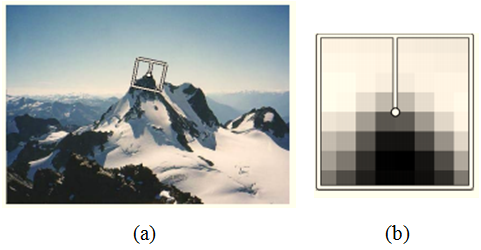
\includegraphics[width=0.45\textwidth]{fig/21.png}
    \vspace{-0.5em} 
    \begin{center}
    \caption{\textcolor{gray}{\footnotesize \textit{
   (a) Et interessepunkt lokaliseret på en bjergtop,  repræsenteret af en firkant, med centrum i interessepunktet og en lodret streg der angiver punktets rotation. (b) Interessepunktet forstørret i et 8x8 pixel område, hvor rotationen af punktet er trukket fra og derfor normaliseret.}}}
    \label{fig:bjerg}
     \end{center}
  \end{figure}
       \vspace{-2.5em}
\noindent
Selv efter kompensering for rotation, skala o.s.v. vil korresponderende regioner stadig variere ift. til hinanden. Udfordringen består derved i at deskriptoren skal være invariant overfor ændringer så korresponderende punkter kan matches korrekt, men også informationsbærende/unikke nok, så der ikke opstår forkerte korrespondancer. Der er mange forskellige måder at beskrive interessepunkter og dertil mange forskellige deskriptorer, der hver især beskriver området forskelligt. I udvælgelsen af en deskriptor skal overvejes følgende:
\begin{itemize}
\item{Hvad skal deskriptoren bruge til at karakterisere området med? Det kan f.eks. være farve, tekstur, gradient orientering el.a.}
\item{Hvor meget information skal deskriptoren indeholde. Dette er ofte defineret ift. hvor stor en dimension vektoren har. Der er her et "trade-of" imellem, hvor beskrivende deskriptoren skal være og hvor lang tid det må tage at udregne deskriptoren da udredningstiden stiger med udvidet kompleksitet.}
\end{itemize}
Ovenstående skal besluttes ift. applikationsdomænet altså, hvad billederne forestiller, og hvor hurtigt deskriptoren skal være at udregne.